%
% Chapter Basic
%
%           Author: Erick Gallesio [eg@kaolin.unice.fr]
%    Creation date:  6-Jan-1993 12:31
% Last file update: 20-May-1995 13:13


\chapter{Basic widgets}

This chapter is devoted to the simplest widgets of the {\stklos} package.
In fact, all the Tk widgets, except the {\em canvas} and {\em text} widgets,
are presented here.

\section{Introduction}

\subsection{A simple interface}

\subsubsection{Defining the widgets}
Before detailing all the simple widgets of the Tk library, we will see how to
build the simple interface which is shown in Figure~\ref{fig-simple-interface}. 
\begin{figure}
\centerline{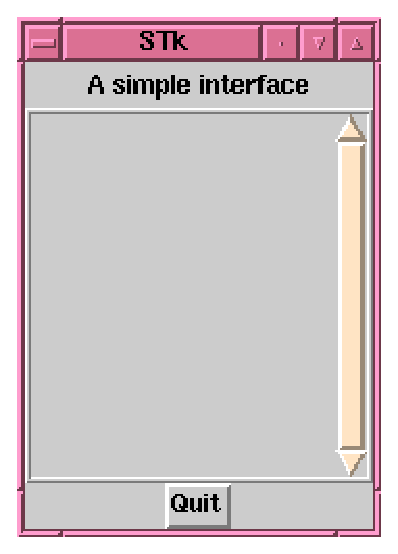
\epsfig{file=Basic-Fig-1.ps}}
\caption{A simple interface}
\label{fig-simple-interface}
\end{figure}
This interface is composed of three main components: 
\begin{enumerate}
\item a label which is situated at top
\item a frame which is itself constituted of two components: 
\begin{enumerate}
\item a listbox, and
\item a scrollbar
\end{enumerate}
\item a ``quit'' button
\end{enumerate}
Let's have look now to  the objects we'll have to create for this interface.
First we can create the top label and the quit button which are relatively
simple. This can be done with the following definitions:
\begin{quote}
\begin{verbatim}
(define lab  (make <Label>  :text "A simple interface"))
(define quit (make <Button> :text "Quit" :command '(exit)))
\end{verbatim}
\end{quote}
The {\tt :command} init-keyword permits to associate an action to the button
(this action will be triggered when the mouse button 1 will be released over
the {\tt quit} button.

The interface shown in Figure~\ref{fig-simple-interface} can be seen as a vertical alignment of
 three components (a label, a listbox with a scrollbar and a button). The
second component is itself an alignment of two object (a scrollbar and a
listbox). What is important to note here is that this alignment is an
horizontal one situated inside a vertical one. In this case, we have to place
the components of our horizontal alignment in a container which acts as a kind
of back box for further layout. The widget which permit to ``embody'' several
widgets is called a frame in the Tk toolkit. Consequently, the listbox and its
scrollbar can be defined by:
\begin{quote}
\begin{verbatim}
(define box  (make <Frame> :border-width 3 :relief "ridge"))
(define l    (make <Listbox>   :parent box))
(define s    (make <Scrollbar> :parent box :orientation "vertical"))
\end{verbatim}
\end{quote}
What is important to note is that the listbox and the scrollbar both tell that
their {\em parent} is the frame {\tt box}. This is this indication which
effectively embody them in the frame.


All the basic components of our interface have been created. What it
rests to do consists to place the graphic components we have just defined
onto screen. First we can map the listbox and its scrollbar in the {\tt
box} object with the {\em packer}\index{packer} geometry manager (see
page \pageref{pack-doc}):
\begin{quote}
\begin{verbatim}
(pack l :expand #t :fill "both" :side "left")
(pack s :expand #t :fill "y" :side "right")
\end{verbatim}
\end{quote}
Both calls to {\tt pack} permit to define the arrangement of the listbox
and the scrollbar into the frame. Here we claim that the scrollbar should
stay on the right side of the frame and that it must expand itself only in
the vertical direction if its containing frame (i.e. {\tt box}) is resized.
Concerning the listbox, it will stay on rigth and it will fill all the
space ({\tt :fill~"both"}) if {\tt box} size changes.

Now we can {\em pack} the three components of this simple interface to show
up them on screen; it can be easily done by:
\begin{quote}
\begin{verbatim}
(pack lab box quit)
\end{verbatim}
\end{quote}
The complete program for the building the previous interface is given in
Figure~\ref{simple:the_code}.

\begin{figure}
{\footnotesize
\begin{verbatim}
;;; Defining the components
(define lab  (make <Label>  :text "A simple interface"))
(define quit (make <Button> :text "Quit" :command '(exit)))
(define box  (make <Frame>  :border-width 3 :relief "ridge"))

;;; Zoom in the box
(define l    (make <Listbox>   :parent box))
(define s    (make <Scrollbar> :parent box :orientation "vertical"))

(pack l :expand #t :fill "both" :side "left")
(pack s :expand #t :fill "y" :side "right")

;;; Pack the components
(pack lab box quit)
\end{verbatim}
}
\caption{Complete code for the simple interface}
\label{simple:the_code}
\end{figure}

\subsubsection{Filling the listbox}

Filling the listbox can be done by calling the {\tt insert}
\index{listbox insert} method. This method permits to add elements in the
listbox. A way to fill the previous lisbox could be:
\begin{quote}
\begin{verbatim}
(insert l 0 "a" "b" "c")
\end{verbatim}
\end{quote}
This will insert 3 lines (containing {\tt "a"}, {\tt "b"} and {\tt "c"})
after the element whose index is 0. Inserting a {\tt "d"} between {\tt "a"}
and {\tt "b"} could be done by the following expression:
\begin{quote}
\begin{verbatim}
(insert l 1 "d")
\end{verbatim}
\end{quote}

Deleting elements of listbox necessitates a call to the {\tt delete}
method. For instance,
\begin{quote}
\begin{verbatim}
(delete l 1)
\end{verbatim}
\end{quote}
deletes the second element of the listbox (first element is at index 0), and
\begin{quote}
\begin{verbatim}
(delete l 0 2)
\end{verbatim}
\end{quote}
permits to delete the three remaining elements. 

{\tt Insert} and {\tt delete} are simple methods built upon Tk commands to
accesss listbox. Most of the time, this way of accessing a listbox is not
too convenient, and it is more easy to see the content of a listbox as its
value. Consequently, the {\tt stklos} {\tt <Listbox>} class defines a
virtual slot\cite{virtual slot} called {\tt value}\index{value} which
permits to read/fill the contents of a listbox as a {\stklos} slot.
For instance, the previous listbox can be filled with:
\begin{quote}
\begin{verbatim}
(set! (value l) '("a" "b" "c"))  ;; or (slot-set! l 'value '(...))
\end{verbatim}
\end{quote}
and the value of the second element of the listbox can be obtained by
\begin{quote}
\begin{verbatim}
(list-ref (value l) 1)
\end{verbatim}
\end{quote}

Of course, the value slot has an initialization keword associated to it,
and the filling of the listbox could have been done during the definition
of the listbox:
\begin{quote}
\begin{verbatim}
(define l (make <Listbox> :parent box 
                          :value  '("a" "b" "c")))
\end{verbatim}
\end{quote}

\subsubsection{Bringing the scrollbar to life}

For now, the lisbox and the scrollbar are disconnected (i.e. moving the
listbox, with {\tt <Shift-Button2>} doesn't move the scrollbar and clicking
the scrollbar does nothing). To make both widgets working accordingly, we have
to associate a command to each widget. First, we can associate a command to
the scrollbar, such as moving it with mouse button will move the listbox. This
can be done with:
\begin{quote}
\begin{verbatim}
(set! (command s) (format #f "y-view ~S " (address-of l)))
\end{verbatim}
\end{quote}
which associates the prefix of a Scheme command to invoke to change the view
in the listbox when the user manipulates the scrollbar. This command is
partial and will be completed effectively when the user will click the
scrollbar (see the <Scrollbar> class description on
page~\pageref{Scrollbar-class} for more details).

This is at  half way of what we have to do for cleanly associate the scrollbar
and the listbox. On the listbox side, we have to associate a command for its 
vertical movement:
\begin{quote}
\begin{verbatim}
(set! (y-scroll-command l) 
      (format #f "scrollbar-set! ~S " (address-of s)))
\end{verbatim}
\end{quote}
Here again, the command associated to the listbox is a partial since it will
be completed by Tk when needed.

As we will see in a next chapter, {\em composite widgets} will permit
to hide all this stuff, and we will be able to define a new class
which will embody a listbox and one (or two) scrollbar.

\subsection{Defining Menus}

\subsubsection{Menu-buttons and Menus}
Tk provides two widgets for building a menu: {\em menubuttons} and
{\em menus}. Those widgets are available through the {\tt
<Menu-button>} and {\tt <Menu>} classes. Instances of {\tt
<Menu-button>} class display a textual string (or a bitmap) and are
associated with an instance of the {\tt <Menu>} class.

\subsubsection{Creating a simple menu bar}

The most current task with menus concerns menu bars
building. {\stklos} provides the convenience function \Indextt{make-menubar}
to ease to the construction of menu bars. To illustrate how this
function work, we'll present the call we must write to produce the
menu bar of Figure~\ref{Menus}.
\begin{figure}
\centerline{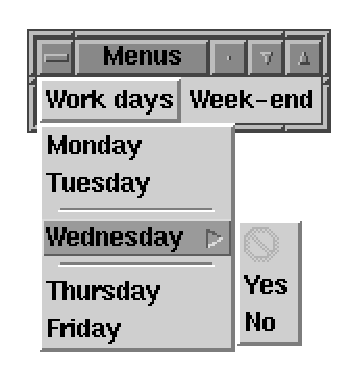
\epsfig{file=Fig2-2.eps}}
\caption{A simple menu}
\label{Menus}
\end{figure}
{\tt Make-menubar} is a function which takes a list of menu buttons
specifications. Each menu button specification is also a list.  First item
of this list is the specification of the menu button; the rest of this list
correspond to the specifaction of the menu items associated to this menu
button. To represent the menu bar of Figure\ref{Menus}, we have a
specification whih looks like:
\begin{quote}
\begin{alltt}
	((Description of {\it Work days} menu button
	     (Fisrt item of {\it Work days})
	     (Second item of {\it Work days}))
	 (Description of {\it Week end} menu button
	     (Fisrt item of {\it Week-end})
	     (Second item of {\it Week-end}))
	)
\end{alltt}
\end{quote}
The complete code for this menu bar is given in Figure\ref{Menus:code}.
Struture of menu buttons and menu items specifications is defined in
\ref{make-menubar}.
\begin{figure}
{\small
\begin{verbatim}
(define l `(("Work days" 
                 ("Monday"    ,(lambda () (format #t "Monday\n")))
                 ("Tuesday"   ,(lambda () (format #t "Tuesday\n")))
                 ("")
                 ("Wednesday"
                     ((command :bitmap error :state disabled)
                      ("Yes" ,(lambda () (format #t "Wednesday (Yes)\n")))
                      ("No"  ,(lambda () (format #t "Wednesday (No) \n")))))
                 ("")
                 ("Thursday"  ,(lambda () (format #t "Thursday\n")))
                 ("Friday"    ,(lambda () (format #t "Friday\n"))))
           ("Week-end"
                 ("Saturday"  ,(lambda () (format #t "Saturday\n")))
                 ("Sunday"    ,(lambda () (format #t "Sunday\n"))))))

(pack (make-menubar *top-root* l))
\end{verbatim}
}
\caption{Code of menu of Figure\ref{Menus}}
\label{Menus:code}
\end{figure}




\section{Simple widgets classes}
%%%%%%%%%%%%%%%%%%%%%%%%%%%%%%%%%%%%%%%%%%%%%%%%%%%%%%%%%%%%%%%%%%%%%%%%%%%%%%
% FRAME
%%%%%%%%%%%%%%%%%%%%%%%%%%%%%%%%%%%%%%%%%%%%%%%%%%%%%%%%%%%%%%%%%%%%%%%%%%%%%%

\subsection{The {\tt Frame} class}

A frame is a {\stklos} simple widget whose primary purpose is to act as a
spacer or container for complex window layouts. A frame object has several
Tk-virtual slots which are listed here:

\begin{ip}

\ITEM{background}
See section \ref{background}.

\ITEM{border-width}
See section \ref{border-width}.

\ITEM{cursor}
See section \ref{cursor}.

\ITEM{height}\label{height}
specifies the desired height for the window. This slot is only
used if the {\em geometry} slots is unspecified. If this pseudo-slot is less than 
or equal to zero (and {\em geometry} is not specified) then the window will 
not request any size at all.

\ITEM{geometry}\label{geometry}
specifies the desired geometry for the widget's window, in the
form {\em width}x{\em height}, where {\em width} is the desired
width of the window and {\em height} is the desired height.  The
units for {\em width} and {\em height} depend on the particular
widget.  For widgets displaying text the units are usually the
size of the characters in the font being displayed;  for other
widgets the units are usually pixels.

\ITEM{relief}
See section \ref{relief}.

\ITEM{width}
specifies the desired width for the window. This slot is only
used if the {\em geometry} slots is unspecified. If this pseudo-slot is less than 
or equal to zero (and {\em  geometry} is not specified) then the window will 
not request any size at all.
\end{ip}

\noindent
Furthermore, the {\em Frame} class admits a special initarg {\tt :class} which
permits to specify the new widget X11 resource class (if the {\tt :class} is
not passed as a parameter during the {\tt make-instance} of the frame, the
widget resource class will be "Frame"). The resource class of a widget can be
specified only at initialization. It can be queried by the {\tt class} reader
but cannot be changed.

Further example use a frame to group three labels in a single object. Here,
the two 
\begin{verbatim}
(setq f (make-instance 'Frame))
(setq l1 (make-instance 'Label :parent f :text " Label 1 " :relief :raised 
                               :map '(:position :left)))
(setq l2 (make-instance 'Label :parent f :text " Label 2 " :relief :raised 
                               :map '(:position :left)))
(setq l3 (make-instance 'Label :text " Label 3 " :relief :raised))
\end{verbatim}

%%%%%%%%%%%%%%%%%%%%%%%%%%%%%%%%%%%%%%%%%%%%%%%%%%%%%%%%%%%%%%%%%%%%%%%%%%%%%%
% LABEL
%%%%%%%%%%%%%%%%%%%%%%%%%%%%%%%%%%%%%%%%%%%%%%%%%%%%%%%%%%%%%%%%%%%%%%%%%%%%%%
\subsection{The label class}

The {\em Label} class defines widgets which are capable to display a textual
string or a bitmap. A label object has several pseudo-slots which are listed here:
\begin{ip}

\ITEM{anchor}\label{anchor}
specifies how the information in a widget (e.g. text or a bitmap) is to be
displayed in the widget. Must be one of the values {\em :n}, {\em :ne}, {\em
:e}, {\em :se}, {\em :s}, {\em :sw}, {\em :w}, {\em :nw}, or {\em `:center}.  For
example, {\em :nw} means display the information such that its top-left corner
is at the top-left corner of the widget.

\ITEM{background}
See section \ref{background}.

\ITEM{bitmap}\label{bitmap}
specifies a string containing the file name of the bitmap to display in the
widget. The exact way in which the bitmap is displayed may be affected by
other slots values such as {\em anchor} or {\em justify}.  Typically, if this
slot is non {\tt nil} is specified then it overrides other pseudo-slots that
specify a textual value to display in the widget; the {\em bitmap} slot may be
reset to an empty string to re-enable a text display.

\ITEM{border-width}
See section \ref{border-width}.

\ITEM{cursor}
See section \ref{cursor}.

\ITEM{font}\label{font}
specifies the font to use when drawing text inside the widget.

\ITEM{foreground}\label{foreground}
specifies the normal foreground color to use when displaying the widget.

\ITEM{height}
specifies a desired height for the label.  If a bitmap is being displayed in
the label then the value is in screen units; for text it is in lines of text.
If this pseudo-slot isn't specified, the label's desired height is computed from
the size of the bitmap or text being displayed in it.

\ITEM{pad-x}\label{pad-x}
specifies a non-negative value indicating how much extra space to request for
the widget in the X-direction. When computing how large a window it needs, the
widget will add this amount to the width it would normally need (as determined
by the width of the things displayed in the widget); if the geometry manager
can satisfy this request, the widget will end up with extra internal space to
the left and/or right of what it displays inside.

\ITEM{pad-y}\label{pad-y}
specifies a non-negative value indicating how much extra space to request for
the widget in the Y-direction. When computing how large a window it needs,
the widget will add this amount to the height it would normally need (as
determined by the height of the things displayed in the widget); if the
geometry manager can satisfy this request, the widget will end up with extra
internal space above and/or below what it displays inside.

\ITEM{relief}
See section \ref{relief}.

\ITEM{text}\label{text}
specifies a string to be displayed inside the widget.  The way in which
the string is displayed depends on the particular widget and may be
determined by other pseudo-slots, such as {\em anchor} or {\em justify}.

\ITEM{text-variable}\label{text-variable}
specifies the name of a variable. The value of the variable is a text
string to be displayed inside the widget; if the variable value changes
then the widget will automatically update itself to reflect the new value.
The way in which the string is displayed in the widget depends on the
particular widget and may be determined by other pseudo-slots, such as
{\em anchor} or {\em justify}. See below how to use this mechanism.

\ITEM{width}
Specifies a desired width for the label. If a bitmap is being displayed in
the label then the value is in screen units; for text it is in characters.  If
this pseudo-slot isn't specified, the label's desired width is computed from the
size of the bitmap or text being displayed in it.

\end{ip}

%%%%%%%%%%%%%%%%%%%%%%%%%%%%%%%%%%%%%%%%%%%%%%%%%%%%%%%%%%%%%%%%%%%%%%%%%%%%%%
% MESSAGE
%%%%%%%%%%%%%%%%%%%%%%%%%%%%%%%%%%%%%%%%%%%%%%%%%%%%%%%%%%%%%%%%%%%%%%%%%%%%%%
\section{The Message class}
The {\em Message} class defines widgets that display a textual string.  A {\em
message}widget has three special features. First, it breaks up its string into
lines in order to produce a given aspect ratio for the window.  The line
breaks are chosen at word boundaries wherever possible (if not even a single
word would fit on a line, then the word will be split across lines).  Newline
characters in the string will force line breaks; they can be used, for
example, to leave blank lines in the display.

The second feature of a message widget is justification.  The text may be
displayed left-justified, centered on a line-by-line basis, or right-justified.

The third feature of a message widget is that it handles control characters
and non-printing characters specially.  Tab characters are replaced with
enough blank space to line up on the next 8-character boundary.  Newlines
cause line breaks.  Other control characters (ASCII code less than hexadecimal
code 20) and characters not defined in the font are displayed as a
four-character sequence \\x{\it hh} where {\it hh} is the two-digit
hexadecimal number corresponding to the character.

\noindent
A message object has several pseudo-slots which are listed here:
\begin{ip}

\ITEM{anchor}
(see section \ref{anchor})

\ITEM{aspect}\label{aspect}
specifies a non-negative integer value indicating desired aspect ratio for the
text. The aspect ratio is specified as 100*width/height. 100 means the text
should be as wide as it is tall, 200 means the text should be twice as wide as
it is tall, 50 means the text should be twice as tall as it is wide, and so
on. Used to choose line length for text if {\em width} pseudo-slot isn't
specified.

\ITEM{background}
(see section \ref{background})

\ITEM{border-width}
(see section \ref{border-width})

\ITEM{cursor}
(see section \ref{cursor})

\ITEM{font}
(see section \ref{font})

\ITEM{justify}\label{justify}
specifies how to justify lines of text. Must be one of {\em :left}, {\em
:center}, or {\em :right}. Defaults to {\em left}. This pseudo-slot works
together with the {\em anchor}, {\em aspect}, {\em padX}, {\em padY}, and {\em
width} pseudo-slots to provide a variety of arrangements of the text within
the window.  The {\em aspect} and {\em width} pseudo-slots determine the
amount of screen space needed to display the text.  The {\em anchor}, {\em
padX}, and {\em padY} pseudo-slots determine where this rectangular area is
displayed within the widget's window, and the {\em justify} pseudo-slot determines
how each line is displayed within that rectangular region.  For example,
suppose {\em anchor} is {\em :e} and {\em justify} is {\em :left}, and that the
message window is much larger than needed for the text. The text will
displayed so that the left edges of all the lines line up and the right edge
of the longest line is {\em pad-x} from the right side of the window; the
entire text block will be centered in the vertical span of the window.
\ITEM{pad-x}
(see section \ref{pad-x})

\ITEM{pad-y}
(see section \ref{pad-y})

\ITEM{relief}
(see section \ref{relief})

\ITEM{text}
(see section \ref{text})

\ITEM{text-variable}
(see section \ref{text-variable})

\ITEM{width}\label{width}
specifies the length of lines in the window. If this pseudo-slot has a value
greater than zero then the {\em aspect} pseudo-slot is ignored and the {\em
width} pseudo-slot determines the line length.  If this pseudo-slot has a
value less than or equal to zero, then the {\em aspect} pseudo-slot determines
the line length.

\end {ip}

%%%%%%%%%%%%%%%%%%%%%%%%%%%%%%%%%%%%%%%%%%%%%%%%%%%%%%%%%%%%%%%%%%%%%%%%%%%%%%
% BUTTON
%%%%%%%%%%%%%%%%%%%%%%%%%%%%%%%%%%%%%%%%%%%%%%%%%%%%%%%%%%%%%%%%%%%%%%%%%%%%%%
\section{The Button class}

The {\em Button} class defines widgets that display a ``reactive'' textual
string or bitmap. It can display itself in either of three different ways,
according to the {\em state} pseudo-slot; it can be made to appear raised,
sunken, or flat; and it can be made to flash.  When a user invokes the button
(defaultly, by pressing mouse button 1 with the cursor over the button), then
the command specified in the {\em command} pseudo-slot is invoked. Several
methods are also defined for buttons. They are presented at end of chapter.

A button object has several pseudo-slots which are listed here:

\begin{ip}

\ITEM{active-background}\label{active-background}
specifies background color to use when drawing active elements.
An element (a widget or portion of a widget) is active if the
mouse cursor is positioned over the element and pressing a mouse button
will cause some action to occur.

\ITEM{active-foreground}\label{active-foreground}
specifies foreground color to use when drawing active elements.
See above for definition of active elements.

\ITEM{anchor}
(see section \ref{anchor})

\ITEM{background}
(see section \ref{background})

\ITEM{bitmap}
(see section \ref{bitmap})

\ITEM{border-width}
(see section \ref{border-width})

\ITEM{command}\label{command}
specifies a command to associate with the button. This command is typically
invoked when mouse button 1 is released over the button window.

\ITEM{cursor}
(see section \ref{cursor})

\ITEM{disabled-foreground}\label{disabled-foreground}
specifies foreground color to use when drawing a disabled element. If the
pseudo-slot is specified as an empty string (which is typically the case on
monochrome displays), disabled elements are drawn with the normal foreground
color but they are dimmed by drawing them with a stippled fill pattern.

\ITEM{font}
(see section \ref{font})

\ITEM{foreground}
(see section \ref{foreground})

\ITEM{height}
specifies a desired height for the button. If a bitmap is being displayed in
the button then the value is in screen units; for text it is in lines of text.
If this pseudo-slot isn't specified, the button's desired height is computed from
the size of the bitmap or text being displayed in it.

\ITEM{pad-x}
(see section \ref{pad-x})

\ITEM{pad-y}
(see section \ref{pad-y})

\ITEM{relief}
(see section \ref{relief})

\ITEM{state}
specifies one of three states for the button:  {\em :normal}, {\em :active},
or {\em `:disabled}.  In normal state the button is displayed using the
{\em foreground} and {\em background} pseudo-slots.  The active state is
typically used when the pointer is over the button.  In active state
the button is displayed using the {\em activeForeground} and
{\em activeBackground} pseudo-slots.  Disabled state means that the button
is insensitive:  it doesn't activate and doesn't respond to mouse
button presses.  In this state the {\em disabledForeground} and
{\em background} pseudo-slots determine how the button is displayed.

\ITEM{text}
(see section \ref{text})

\ITEM{text-variable}
(see section \ref{text-variable})

\ITEM{width}
Specifies a desired width for the button.  If a bitmap is being displayed in
the button then the value is in screen units;for text it is in characters.  If
this option isn't specified, the button's desired width is computed from the
size of the bitmap or text being displayed in it.

\end {ip}
\noindent
{\em Example}
The following example show a simple use of buttons. 
{\tt 
\begin{quote}
\begin{verbatim}
(setq b1 (make-instance 'Button :text "Yes" 
                                :command '(format t "You said Yes")))
(setq b2 (make-instance 'Button :text "No"
                                :command '(format t "You said No")))
(event-loop)
\end{verbatim}
\end{quote}}

%anchor
%background
%bitmap
%borderwidth
%cursor
%font
%foreground
%pad-x
%pad-y
%relief
%text
%text-variable

\section {Functions of this chapter}

